% !TEX root = ../Documentation.tex

\subsection{System overview (R-M)}
The requirements of the new parser have been described in the project planning \citenac{plan}.
Basically, both the old and the new parser must be able to make a conversion from a text file (ADL-script) to a parse tree (the P-structure).
\autoref{fig:data-flow-1} depicts this data flow.
%
\begin{figure}[htb!]
	\centering
	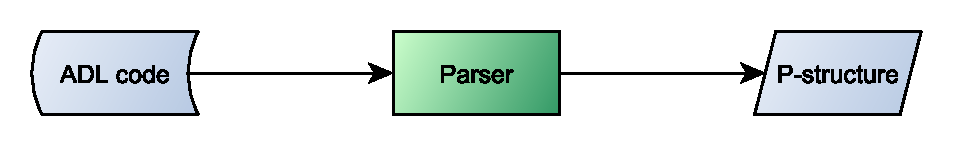
\includegraphics[width=0.586\textwidth]{Figures/DataFlow1}
	\caption{Relevant data flow for the Ampersand parsing component}
	\label{fig:data-flow-1}
\end{figure}

Often, the parsing component is separated into a lexer (that converts text to tokens) and the actual parser (that converts the tokens into the parse tree).
Since this separation is considered beneficial for both maintainability and performance \citeac{parsec}, we assumed from the beginning that the new Ampersand parser would be separated in this way.
This is depicted in \autoref{fig:data-flow-2}.
The previous parser also had a separate lexer, but the name was scanner instead.
%
\begin{figure}[htb!]
	\centering
	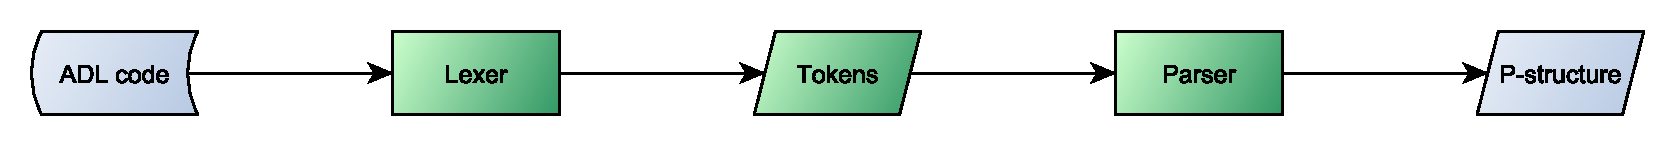
\includegraphics[width=1\textwidth]{Figures/DataFlow2}
	\caption{Data flow for the Ampersand lexing and parsing components}
	\label{fig:data-flow-2}
\end{figure}

In order to take the next steps and understand how the parser can be designed, we first take a look at the grammar in \autoref{subsec:analysis-grammar} and the parse tree in \autoref{subsec:analysis-parse-tree}.
Afterwards, we analyze the lexer with the original token structure, so that we can define a new token structure, in \autoref{subsec:analysis-lexer}.
Finally, we analyze the parser in \autoref{subsec:analysis-parser} and the generated errors in \autoref{subsec:analysis-errors}.
